% ============================================================
%  Chapter 1 — Introduction
% ============================================================
\chapter{Introduction}
\label{ch:intro}

% NOTE: paraphrase of the central observation of Land's Retinex work, not a
%       verbatim quotation — attributed accordingly.
\myquotation{%
A photograph does not record what things look like.
It records how light from those things reached the camera at one specific moment.}{%
after Edwin Land}

When we look at a red apple under a warm yellow lamp, we still see a red apple.
Our visual system separates the colour of the apple's skin from the colour of the
light hitting it.
This ability, called \emph{colour constancy}, is so automatic in humans that
we rarely think about it.
For computers, it is a hard problem.
A camera simply records the product of surface colour and illumination, and the two
are mixed together in every pixel.
Separating them is the goal of \emph{Intrinsic Image Decomposition} (IID).

IID has a long history in computer vision and colour science, dating back to the
Retinex theory of \mycitetext{land71retinex}.
The core idea is that a photograph $\mathbf{I}$ can be modelled as the product of
two layers: an \emph{albedo} $\mathbf{A}$ and a \emph{shading} $S$.
\begin{equation}
  \mathbf{I}(p) = \mathbf{A}(p) \cdot S(p), \qquad \forall\, p \in \Omega
  \label{eq:iid_model}
\end{equation}
Here $p$ denotes a pixel, $\Omega$ is the set of all pixels, the albedo encodes
the true material colour at each pixel, and the shading encodes how bright the
surface is due to lighting and geometry.
If we can recover $\mathbf{A}$ reliably, we obtain a lighting-independent
description of the scene. This separation has practical consequences. An
interior-design tool can recolour a wall without painting over its shadows; an
augmented-reality system can place a virtual chair under the room's existing
light; a photograph can be re-lit without changing the apparent material; and a
catalogue or inspection system can compare product colours captured under
different lamps. All four applications fail when lamp colour remains baked into
the estimated material.

\begin{figure}[t!]
  \centering
  \begin{minipage}[t]{0.235\textwidth}\centering
    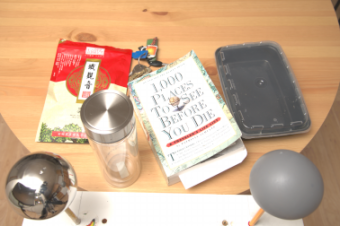
\includegraphics[width=\linewidth]{images/arch/input.png}\\[-1mm]
    \small Observed image $\mathbf{I}$
  \end{minipage}\hfill
  \begin{minipage}[t]{0.235\textwidth}\centering
    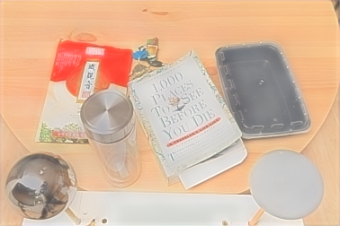
\includegraphics[width=\linewidth]{images/arch/albedo.png}\\[-1mm]
    \small Material albedo $\mathbf{A}$
  \end{minipage}\hfill
  \begin{minipage}[t]{0.235\textwidth}\centering
    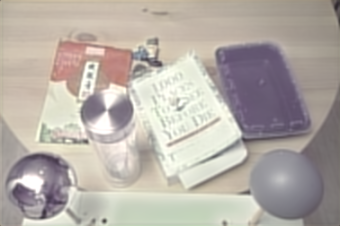
\includegraphics[width=\linewidth]{images/arch/shading.png}\\[-1mm]
    \small Diffuse shading $\mathbf{S}_d$
  \end{minipage}\hfill
  \begin{minipage}[t]{0.235\textwidth}\centering
    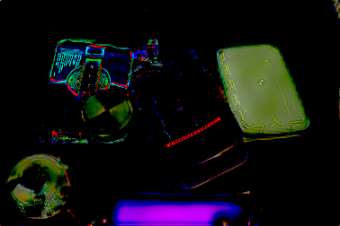
\includegraphics[width=\linewidth]{images/arch/residual.png}\\[-1mm]
    \small Non-diffuse residual $\mathbf{R}$
  \end{minipage}
  \caption[Visual meaning of an intrinsic decomposition.]{%
    Visual meaning of the decomposition used in this thesis. The photograph is
    explained by material colour multiplied by the illumination arriving at each
    surface, plus a residual for effects such as highlights and visible light
    sources. These are illustrative predictions, not separate photographs.
  }
  \label{fig:intro_layers}
\end{figure}


\section{The Coloured Illumination Problem}

Most IID methods, both classical and modern, share an implicit assumption:
the illuminant is grey.
Under a grey illuminant, the shading $S$ in \eqnref{eq:iid_model} is a single
scalar value per pixel, and colour information in the image comes entirely from
the albedo.
This simplification allows the model to be trained with standard supervision,
and it works well when the light is close to white.

Real indoor scenes, however, rarely have pure white light.
Incandescent bulbs emit warm orange-yellow light; fluorescent tubes lean green;
LEDs can be cool blue; afternoon sunlight through a window can have a strong
orange cast.
When illumination is coloured, the shading is no longer achromatic because it carries
a hue, and the simple product model in \eqnref{eq:iid_model} breaks down.
What typically happens is that the model absorbs the illuminant colour into the
albedo, because the albedo is the only 3-channel (RGB) term in the equation.
The result is that the same wall looks orange when lit by one lamp and blue
when lit by another, even though its paint has not changed.

This is not a failure of any specific model; it is a fundamental ambiguity.
Without additional constraints, there is no way to tell from a single image
whether the orange hue in a pixel comes from orange paint or orange light.
The state of the art handles this by training on large synthetic datasets with
diverse illumination, which provides statistical regularisation, but it does not
resolve the core ambiguity.
\figref{fig:intro_constancy} shows a concrete example: two photographs of the
same indoor scene lit by different coloured lamps.
A model trained without illuminant-invariance constraints assigns different albedos
to the same wall in each image, while our approach, detailed in this report, keeps
the predicted albedo stable.

\begin{figure}[t!]
  \centering
  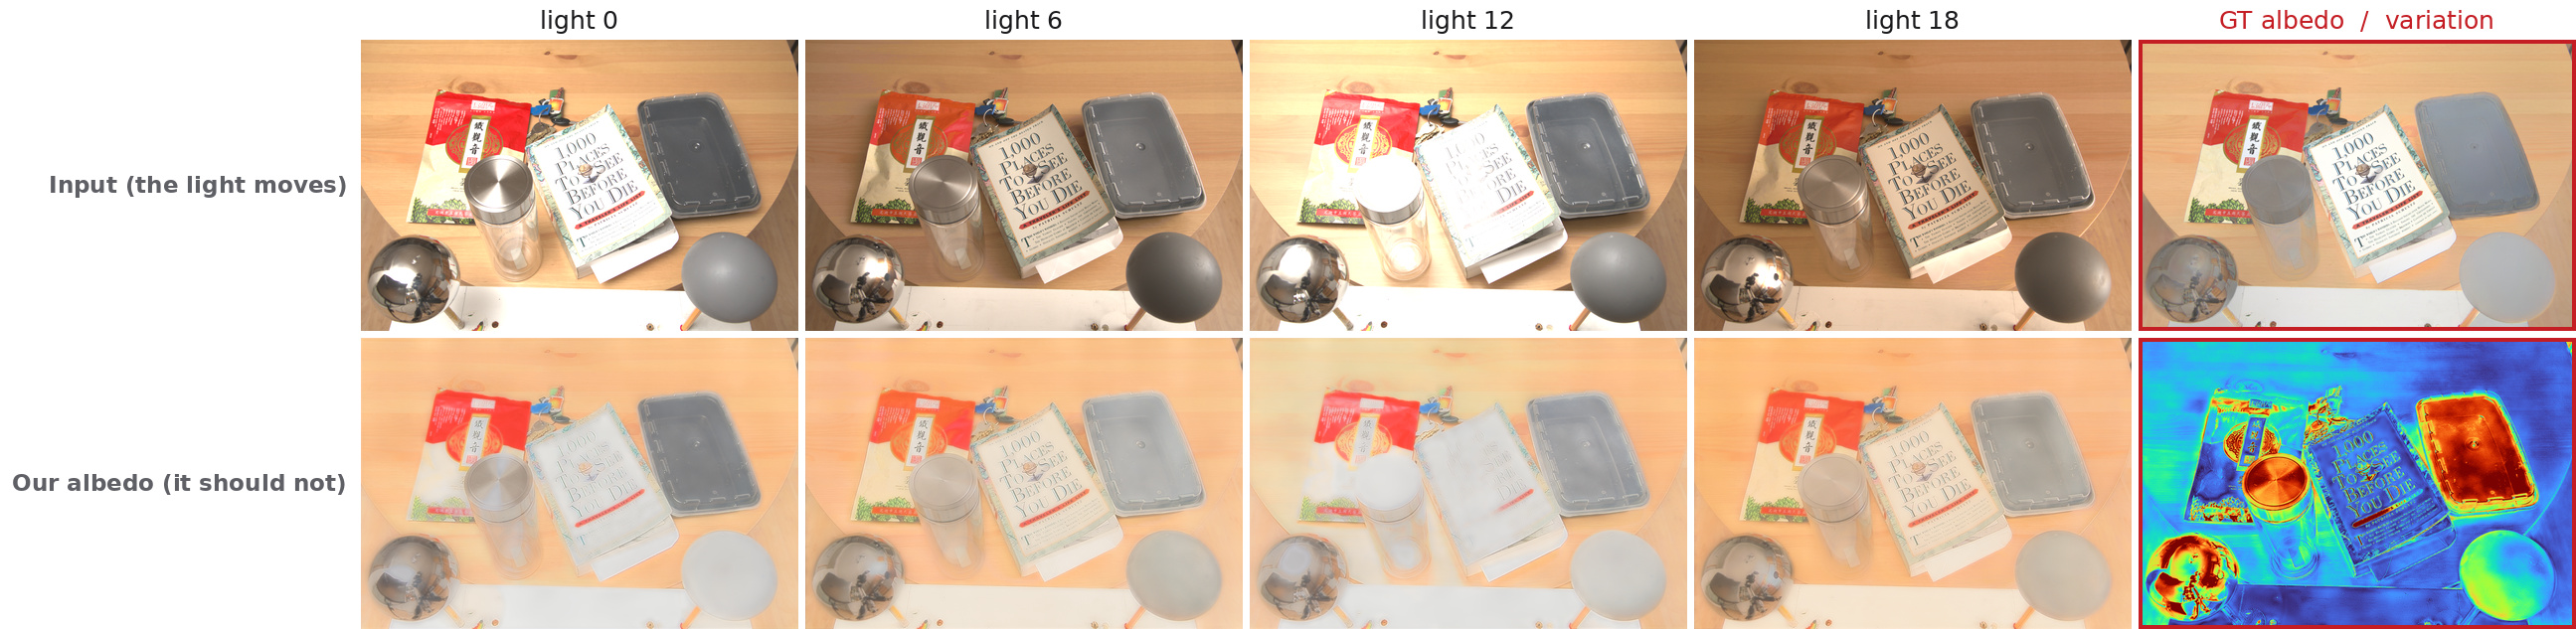
\includegraphics[width=\textwidth]{images/hires/mid_ours.jpg}
  \caption[MID albedo constancy under four illuminants.]{%
    Albedo predictions on one MID scene under four light conditions.
    The upper row shows the four inputs and the dataset pseudo-ground-truth albedo;
    the lower row shows the four predictions and a per-pixel coefficient-of-variation
    map (red marks regions that change with the light).
    The predicted albedo stays consistent as the illumination changes, so the
    CoV maps remain cool over the flat surfaces where the colour cast varies
    most: the constancy this thesis targets.
  }
  \label{fig:intro_constancy}
\end{figure}


\section{Our Approach: Cross-Render Albedo Invariance}

We attack the coloured illumination problem through a training-time constraint
we call \emph{Cross-Render Albedo Invariance} (CARI).
The idea is straightforward: if a dataset contains images of the same physical
scene photographed under different coloured illuminants, then a correct IID model
must produce the same albedo for all of those images.
We can enforce this with a loss term that directly penalises any change in the
predicted albedo across the illuminant conditions.
At the same time, a companion loss ensures that the shading layer absorbs and
explains the difference between the two images, so the model cannot simply predict
a flat albedo and ignore the image content.

To apply CARI in practice, we need a dataset with real multi-illuminant pairs.
We use the Multi-Illumination Dataset (MID), which contains indoor scenes photographed
under several different light sources.
A crucial practical insight arises here: most datasets pre-process images with
\emph{white balance} (WB), which neutralises the illuminant colour and produces
images that all look as if they were lit by white light.
This pre-processing is counterproductive for our goal.
CARI needs the illuminant colour to be visible in the images so the model can
learn to separate it from the material colour.
We therefore train on raw, un-white-balanced MID pairs, preserving the full
illuminant information in the training signal.

We implement CARI inside a model built on a frozen \emph{DINOv2-Large}
vision encoder \mycite{oquab24dinov2} and a Dense Prediction Transformer (DPT)
decoder \mycite{ranftl21dpt}.
The model is first trained on Hypersim \mycite{roberts21hypersim}, a large
photorealistic synthetic dataset with ground truth albedo and shading, which gives
it a strong baseline decomposition.
CARI losses are then added in a second stage, using the MID raw pairs to push
the model toward illuminant-invariant albedo predictions.


\section{Contributions}

The main contributions of this work are:

\begin{itemize}

  \item \textbf{Cross-Render Albedo Invariance (CARI).}
  We introduce paired invariance and explanation losses that require the same
  scene to retain its albedo while shading explains the change of illumination.

  \item \textbf{A raw-pair training result.}
  Controlled ablations show that white balancing removes much of the colour
  variation needed by CARI; retaining raw MID pairs materially improves the
  targeted constancy measures.

  \item \textbf{A corrected evaluation of colour constancy.}
  We show that a pooled chroma-cast score can reward desaturated albedo, then
  separate cross-light invariance from calibration to a pseudo-albedo reference.
  Four complementary benchmarks report real constancy, measured colour,
  synthetic dense accuracy, and perceptual reflectance ordering.

  \item \textbf{3D-Front-IID and an informative negative result.}
  We render 5{,}056 paired observations with deliberately varied illuminant
  colour and exact albedo. The corpus improves the colour axis it covers but not
  ARAP's hard-shadow failure mode, exposing a specific gap in the renderer rather
  than hiding a null result.

  \item \textbf{Optimisation evidence.}
  The final refinement study documents the measured trade-off between invariant
  material colour, hard-shadow leakage, and retained image structure.

\end{itemize}

The project code, training configurations, and evaluation scripts are publicly available at
\url{https://github.com/tmkhang1999/CARI}.

The rest of this report is organised as follows.
\chapref{ch:related} reviews related work on IID, multi-illuminant scenes, and
the datasets used for evaluation.
\chapref{ch:method} describes the model architecture and the CARI training
strategy.
\chapref{ch:implementation} covers the loss terms, training data, and optimisation
schedule in detail.
\chapref{ch:experiments} presents quantitative and qualitative experiments on
all four benchmarks, together with the ablation studies and a controlled
negative result.
\chapref{ch:practice} demonstrates qualitative factor edits built directly on the
decomposition: residual suppression and factor-space illumination adjustment.
\chapref{ch:conclusion} summarises the findings, discusses limitations, and
outlines directions for future work.
